% !TeX encoding = UTF-8
% !TeX program = xelatex
% !TeX spellcheck = en_US

\documentclass[degree=master]{ustcthesis}
\usepackage{hyperref}
\usepackage{float} % 必须加这个，因为你的图片排版用了 [H] 参数

\newcommand{\projectname}{HarmonyOS Transparent Bubble Rendering - Thin Film + DBSTT}
\newcommand{\codepath}[1]{\texttt{#1}}
\newcommand{\reportfigure}[4]{%
  \begin{figure}[H]
    \centering
    \IfFileExists{figures/#1}{%
      \includegraphics[width=#2\linewidth]{figures/#1}%
    }{%
      \fbox{%
        \begin{minipage}[c][#3][c]{0.88\linewidth}
          \centering
          \texttt{\detokenize{#1}}\\[0.8em]
          截图占位：#4
        \end{minipage}
      }%
    }
    \caption{#4}
  \end{figure}
}
% degree      = doctor | master | bachelor
% degree-type = academic | professional
% language    = chinese | english
% fontset     = windows | mac | ubuntu | fandol

% 加载宏包、全部的配置
\input{ustcsetup.tex}
\lstset{
  basicstyle=\ttfamily\small,
  breaklines=true,
  columns=fullflexible,
  keepspaces=true
}


\begin{document}

\maketitle


% !TeX root = ../main.tex

\ustcsetup{
  keywords = {
    肥皂泡渲染，HarmonyOS，屏幕空间折射，薄膜干涉，虹彩，泡泡形变仿真，OpenGL ES
  },
  keywords* = {
    soap bubble rendering, HarmonyOS, screen-space refraction,
    thin-film interference, iridescence, Bubble Simulation, OpenGL ES
  },
}

\begin{abstract}
  本项目面向【CCF CAD/CG 2026】高质量实时渲染技术挑战赛赛题二“基于鸿蒙的透明物体实时色散渲染系统”，实现了一个运行于 HarmonyOS 设备上的透明泡泡实时渲染与交互系统。系统采用 HarmonyOS ArkTS + XComponent + NAPI + C++ OpenGL ES 3.0 的整体架构，以屏幕空间折射为核心，通过多阶段 FBO 合成近似肥皂泡的双界面折射；在材质上实现了 Kim2012 的实时薄膜干涉计算模式以及 Belcour Airy 风格的多波长薄膜反射模式；在动态与交互上实现了基于噪声和排液趋势的膜厚变化、触摸驱动的局部扰动与波纹、主泡泡的 DBSTT/vortex sheet 表面形变，以及多展示泡泡的漂移组织与参数面板控制。本文按照渲染管线、光学模型、交互实现与动态模拟的顺序介绍最终初赛提交版本的系统设计、关键实现与局限。 
\end{abstract}

\begin{abstract*}
  This project targets Track 2, “Real-Time Dispersion Rendering of Transparent
  Objects on HarmonyOS,” and implements a real-time transparent bubble
  rendering and interaction system on HarmonyOS devices. The final system is
  built with HarmonyOS ArkTS, XComponent, NAPI, and C++ OpenGL ES 3.0.
  Multi-stage framebuffer composition is used to approximate two-interface
  refraction, the renderer supports three iridescence modes named Kim2012 and Belcour Airy, and the interactive demo includes
  procedural film-thickness variation, touch-driven local disturbance,
  DBSTT/vortex-sheet-inspired deformation for the main bubble, and multiple
  drifting display bubbles with a real-time parameter panel. This report
  directly presents the final HarmonyOS submission, including its rendering
  pipeline, optical models, interaction design, simulation method, and current
  limitations.
\end{abstract*}


\tableofcontents


\mainmatter
\chapter{引言}

\section{赛题目标与总体结构}

赛题二“基于鸿蒙的透明物体实时色散渲染系统”要求参赛者在给定基线工程上完成透明物体的实时折射、色散与交互展示，并进一步体现多泡泡效果、运动模拟、完整 UI 和稳定运行能力。肥皂泡恰好同时包含透明折射、薄膜干涉、动态表面和交互反馈四类典型问题，因此非常适合作为赛题落地对象。

本技术文档将介绍本队最终决赛提交版本的核心技术路线。决赛版本在初赛基础上，将系统从"单主泡泡+装饰展示泡泡"架构扩展为完整的多泡泡交互系统：泡泡之间可以动态接触、形成共享膜、融合吸收或分离，并支持运行时增删泡泡与方向性风场。实现上，系统被组织为渲染管线、薄膜材质、几何数据、动态模拟和资源加载几个相对独立的模块，并通过 ArkTS 页面层与 Native 渲染层共同完成最终应用。

\reportfigure{1.1.jpg}{0.44}{0.28\textheight}{最终整体效果：多泡泡交互场景，包含背景折射、天空盒环境、虹彩边缘与泡泡间接触共享膜。}

\section{系统组成}

最终鸿蒙提交版本的核心源码位于：
\begin{quote}
  \path{HarmonyOS_Source_Submission/refraction/}
\end{quote}
下表列出了和实现相关的各个模块。

\begin{table}[H]
  \centering
  \caption{系统模块与职责}
  \label{tab:structure}
  \begin{tabular}{p{0.22\linewidth}p{0.30\linewidth}p{0.36\linewidth}}
    \toprule
    模块 & 主要内容 & 作用 \\
    \midrule
    页面与交互 & ArkTS 页面、XComponent、按钮与参数面板 & 承载渲染画面，处理触控输入、模式切换、状态显示和参数调节。\\
    Native 接口与管线 & NAPI、EGL、FBO、绘制顺序 & 连接 ArkTS 与 C++ 渲染层，组织多阶段折射渲染和场景合成。\\
    泡泡材质 & 折射 shader、薄膜虹彩、动态膜厚 & 实现屏幕空间折射、Kim2012/LUT/Belcour Airy 三种虹彩模式和触摸波纹。\\
    渲染封装 & 相机、模型、网格、shader 工具类 & 管理天空盒、球体、动态网格和 OpenGL ES 绘制细节。\\
    表面模拟 & DBSTT/vortex sheet 单泡泡动态 & 让主泡泡轮廓和法线随时间产生轻微形变。\\
    \midrule
    多泡泡交互 & 接触图、空间哈希、表面控制点、共享膜 & 管理泡泡间接触检测、接触圆动力学、持久表面变形、共享膜生成与弯曲、融合/分离事件。\\
    风场与动态管理 & 方向性风场、动态增删泡泡 & 提供可调节的全局风场，支持运行时按需创建和删除泡泡。\\
    资源文件 & 天空盒、薄膜 LUT、HAP 提交资源 & 提供环境反射、背景折射参照、预计算薄膜反射数据和移动端运行素材。\\
    \bottomrule
  \end{tabular}
\end{table}

\section{运行环境}

本项目初期开发在 Windows 主机上进行，验证设计可行性和效果后使用 DevEco Studio 完成基于 HarmonyOS 架构的实现。推荐环境如下：

\begin{table}[H]
  \centering
  \caption{推荐编译与运行环境}
  \begin{tabular}{p{0.28\linewidth}p{0.58\linewidth}}
    \toprule
    项目 & 要求 \\
    \midrule
    开发主机操作系统 & Windows 11。\\
    开发工具 & DevEco Studio 6.0.2。\\
    SDK 环境 & HarmonyOS SDK 6.0.2（API 22）。\\
    页面层 & ArkTS + XComponent。\\
    Native 层 & CMake + C++ + EGL + OpenGL ES 3.0 + NAPI。\\
    真机测试 & 华为 Mate 70 Pro（HarmonyOS 6.0，API 22）。\\
    模拟器 & HarmonyOS 本地模拟器。\\
    \bottomrule
  \end{tabular}
\end{table}

命令行构建可使用 Hvigor，例如：

\begin{lstlisting}[language=bash]
node "E:\huawei\DevEco Studio\tools\hvigor\bin\hvigorw.js" assembleHap --no-daemon
\end{lstlisting}

签名完成后，构建产物通常位于：
\begin{quote}
  \path{entry/build/default/outputs/default/entry-default-signed.hap}
\end{quote}
提交的文件中已经整理出 \codepath{HarmonyOS\_Source\_Submission} 下的“可执行程序”目录。

\chapter{渲染管线设计}
\section{渲染管线}

\subsection{多阶段屏幕空间折射}

实时折射如果完全按路径追踪计算，需要跟踪光线穿过薄膜前表面、后表面以及环境的多次传播，开销较大。项目采用 Wyman 的 image-space refraction 思路 \cite{wyman2005refraction}：先把可被折射的背景渲染成纹理，再在泡泡 shader 中根据法线和视线方向扰动采样坐标，从而得到近似折射效果。为了在鸿蒙端同时组织主泡泡、展示泡泡和前后景关系，系统在 Native 层采用多阶段 FBO 合成，但核心光学思路仍然是用两个屏幕空间界面近似肥皂泡的双界面折射。

\begin{figure}[H]
  \centering
  
\includegraphics[width=0.92\linewidth]{pipeline_pic2.jpeg}
  \caption{屏幕空间折射主线与多阶段 FBO 合成关系。}
  \label{fig:pipeline}
\end{figure}

这一主线被组织为以下几个连续阶段：

\begin{enumerate}
  \item \textbf{背景阶段}：将天空盒和背景参照物渲染到 \codepath{backgroundFBO}。
  \item \textbf{后景阶段}：把主泡泡后方场景写入 \codepath{sceneBehindFBO}，为背面折射提供输入。
  \item \textbf{背面阶段}：开启正面剔除，只绘制主泡泡背面，并输出到 \codepath{backFaceFBO}。
  \item \textbf{主场景阶段}：绘制包含交互泡泡的场景到 \codepath{mainSceneFBO}，供后续合成采样。
  \item \textbf{最终合成阶段}：将所有泡泡合成到 \codepath{finalSceneFBO}，再输出到屏幕。
\end{enumerate}

这种方法的优点是完全运行在 GPU rasterization 管线中，不需要逐像素射线求交；缺点是折射对象必须已经出现在屏幕空间纹理中，因此它是视觉上可信的近似，而不是严格物理光线追踪。对于鸿蒙终端场景而言，这种取舍能够在移动端预算下同时满足折射观感、多泡泡层次和交互响应速度。

\subsection{FBO 尺寸策略与坐标修正}

系统在 \codepath{InitFBO} 中采用低分辨率 FBO 合成，再由全屏四边形放大到最终屏幕，以兼顾移动端性能与画面完整性。其核心策略可写为：

\[
W_{\mathrm{fbo}} = 0.5 W_{\mathrm{screen}}, \qquad
H_{\mathrm{fbo}} = 0.5 H_{\mathrm{screen}}.
\]

由于 FBO 分辨率与窗口分辨率不同，正面渲染到屏幕时，\codepath{gl\_FragCoord} 是窗口像素坐标；背面渲染到 FBO 时，\codepath{gl\_FragCoord} 是 FBO 像素坐标。项目通过 \codepath{uRenderToFBO} 区分两种情况：

\begin{lstlisting}[language=C++]
vec2 fboPixel = (uRenderToFBO == 1)
    ? screenPixel
    : screenPixel * (uFBOSize / uWinResolution);
\end{lstlisting}

该修正对多泡泡渲染尤其重要。各泡泡在不同 pass 中复用同一套折射与虹彩 shader，如果输入坐标不能正确映射到 FBO 空间，就会出现采样越界或局部发黑。修正后，所有交互泡泡都沿用统一材质逻辑，并通过模型矩阵、局部几何扰动强度、虹彩模式、输出透明度以及是否响应交互等参数来区分。

\section{屏幕空间折射实现}

\subsection{折射方向}

在 fragment shader 中，入射方向取视线方向 \codepath{eye}，法线取世界法线 \codepath{normal}。肥皂液近似水的折射率，程序使用

\[
\eta = \frac{n_{\mathrm{air}}}{n_{\mathrm{film}}} = \frac{1.0}{1.33}.
\]

GLSL 中调用 \codepath{refract(eye, normal, eta)} 得到折射方向，并转换到视图空间：

\begin{lstlisting}[language=C++]
vec3 refractVec = mat3(vView) * refract(eye, normal, iorRatio);
\end{lstlisting}

随后取折射方向的 $xy$ 分量作为屏幕空间偏移方向。因为这是屏幕空间近似，shader 并不计算真实光线与后表面的三维交点，而是把折射方向转化为背景纹理采样偏移。

\subsection{边缘增强与薄膜厚度影响}

肥皂泡的中心通常接近透明，轮廓处视觉效果更明显。程序用

\[
e = 1 - |\mathbf{V}\cdot\mathbf{N}|
\]

表示边缘程度，其中 $\mathbf{V}$ 是视线方向，$\mathbf{N}$ 是表面法线。随后通过 \codepath{smoothstep} 得到更平滑的边缘曲线：

\[
e_{\mathrm{profile}} = \mathrm{smoothstep}(0.18, 0.92, e).
\]

折射偏移的核心形式可写为：

\[
\Delta \mathbf{p}
= \mathbf{T}_{xy}\,
s_{\mathrm{ref}}\,
s_{\mathrm{face}}\,
s_{\mathrm{film}}\,
r_{\mathrm{px}}\,
s_{\mathrm{edge}}\,
s_{\mathrm{touch}},
\]

其中 $\mathbf{T}_{xy}$ 是视图空间折射方向的屏幕分量，$s_{\mathrm{ref}}$ 是用户可调的 \codepath{uRefractionStrength}，$s_{\mathrm{face}}$ 区分正面和背面，$s_{\mathrm{film}}$ 由薄膜厚度和边缘程度共同决定，$r_{\mathrm{px}}$ 是泡泡屏幕半径，$s_{\mathrm{edge}}$ 是边缘增强。

背面 pass 使用更小的折射强度：

\[
s_{\mathrm{face}} =
\begin{cases}
0.16, & \text{背面 pass},\\
1.0, & \text{正面 pass}.
\end{cases}
\]

这样做可以避免双界面叠加时背景被过度扭曲。最终偏移还会被 \codepath{uMaxOffsetRatio} 限制在泡泡屏幕半径的一定比例内，防止采样跳变。

\reportfigure{2.2.jpg}{0.5}{0.26\textheight}{背景小球经过主泡泡后的折射扭曲效果}

\section{薄膜虹彩模型}

\subsection{薄膜干涉基础}

肥皂泡薄膜的厚度通常为数百纳米，和可见光波长处在同一数量级。光线在空气--薄膜界面与薄膜--空气界面发生反射，两个反射波之间产生光程差。对某一波长 $\lambda$，相位差可写为：

\[
\phi_\lambda =
\frac{4\pi n d \cos\theta_t}{\lambda},
\]

其中 $n$ 是薄膜折射率，$d$ 是薄膜厚度，$\theta_t$ 是薄膜内部折射角。不同波长的反射强度随 $\phi_\lambda$ 改变，因此 RGB 颜色会随厚度、视角和法线方向变化。

项目中所有虹彩模式都使用动态厚度 $d$ 与视角项 $|\mathbf{V}\cdot\mathbf{N}|$ 作为输入，但三种模式计算反射率的方式不同。

\subsection{Kim2012 模式：实时 RGB 波长采样}

程序界面中的 \textbf{Kim2012} 模式对应 \codepath{uIridescenceMode = 0}。它参考 Kim 与 Park 关于实时肥皂泡虹彩渲染的做法 \cite{kim2012soapbubble}，在 shader 中直接计算薄膜对 RGB 三个代表波长的反射率。实现文件为 \codepath{shader\_refraction.h} 中的：

\begin{itemize}
  \item \codepath{fresnelCoefficients}
  \item \codepath{interferencePhase}
  \item \codepath{thinFilmReflectance}
  \item \codepath{kim2012Iridescence}
\end{itemize}

对每个波长，程序先计算 s 偏振和 p 偏振的 Fresnel 振幅系数，再用相位差得到反射率近似：

\[
R_\lambda =
\frac{r_s^2(1-\cos\phi)}{1+r_s^4-2r_s^2\cos\phi}
+
\frac{r_p^2(1-\cos\phi)}{1+r_p^4-2r_p^2\cos\phi}.
\]

当前版本采样的三个代表波长为：

\[
\lambda_R=615\mathrm{nm},\quad
\lambda_G=535\mathrm{nm},\quad
\lambda_B=465\mathrm{nm}.
\]

该模式的优点是公式直接、易解释，能清楚体现薄膜厚度和相位差对颜色的影响；不足是只用三个波长代表完整可见光谱，边缘颜色可能更鲜艳，也更容易出现强烈的 RGB 分离。


\subsection{Belcour Airy 模式：多波长 Airy 反射近似}

\textbf{Belcour Airy} 模式对应 \codepath{uIridescenceMode = 2}，也是当前默认模式。它参考 Belcour 与 Barla 对薄膜虹彩和 Airy reflectance 的建模思想 \cite{belcour2017iridescence}，但本项目没有完整实现论文中的微表面解析预积分，而是在肥皂泡 shader 中实现了一个面向移动端实时展示的简化 Airy 反射模型。

对某一偏振方向，薄膜多次内反射的复振幅可写为：

\[
A_\lambda =
r_{12}
+
\frac{t_{12}r_{23}t_{21}e^{i\phi_\lambda}}
{1-r_{21}r_{23}e^{i\phi_\lambda}},
\qquad
R_\lambda = |A_\lambda|^2.
\]

程序分别计算 s、p 两个偏振方向，再取平均。随后在 \codepath{belcourAiryWeightedIridescence} 中采样多个波长：

\[
430, 470, 500, 535, 575, 615, 650 \mathrm{nm}.
\]

这些波长再乘以经验 RGB 权重得到最终颜色。相比 Kim2012 模式，Belcour Airy 模式的颜色更平滑，环境反射也会被薄膜反射率染色，因此更适合作为最终鸿蒙版本的默认外观。

\subsection{不同模式对比}

\begin{table}[H]
  \centering
  \caption{不同虹彩模式的区别}
  \label{tab:modes}
  \begin{tabular}{p{0.18\linewidth}p{0.25\linewidth}p{0.23\linewidth}p{0.23\linewidth}}
    \toprule
    模式 & 计算方式 & 优点 & 局限 \\
    \midrule
    Kim2012 & shader 中实时计算 RGB 三个代表波长的薄膜干涉反射率。 & 公式直观，便于说明相位差、Fresnel 系数和厚度的关系。 & 只采样三个波长，颜色可能偏强，光谱连续性有限。\\
    Belcour Airy & 使用 Airy 风格的多次内反射公式，并采样多个波长加权合成。 & 颜色过渡更平滑，边缘和环境反射更自然，是当前默认模式。 & 是项目级简化实现，不是完整 Belcour 微表面预积分模型。\\
    \bottomrule
  \end{tabular}
\end{table}

\begin{figure}[H]
  \centering
  \begin{minipage}[t]{0.32\linewidth}
    \centering
    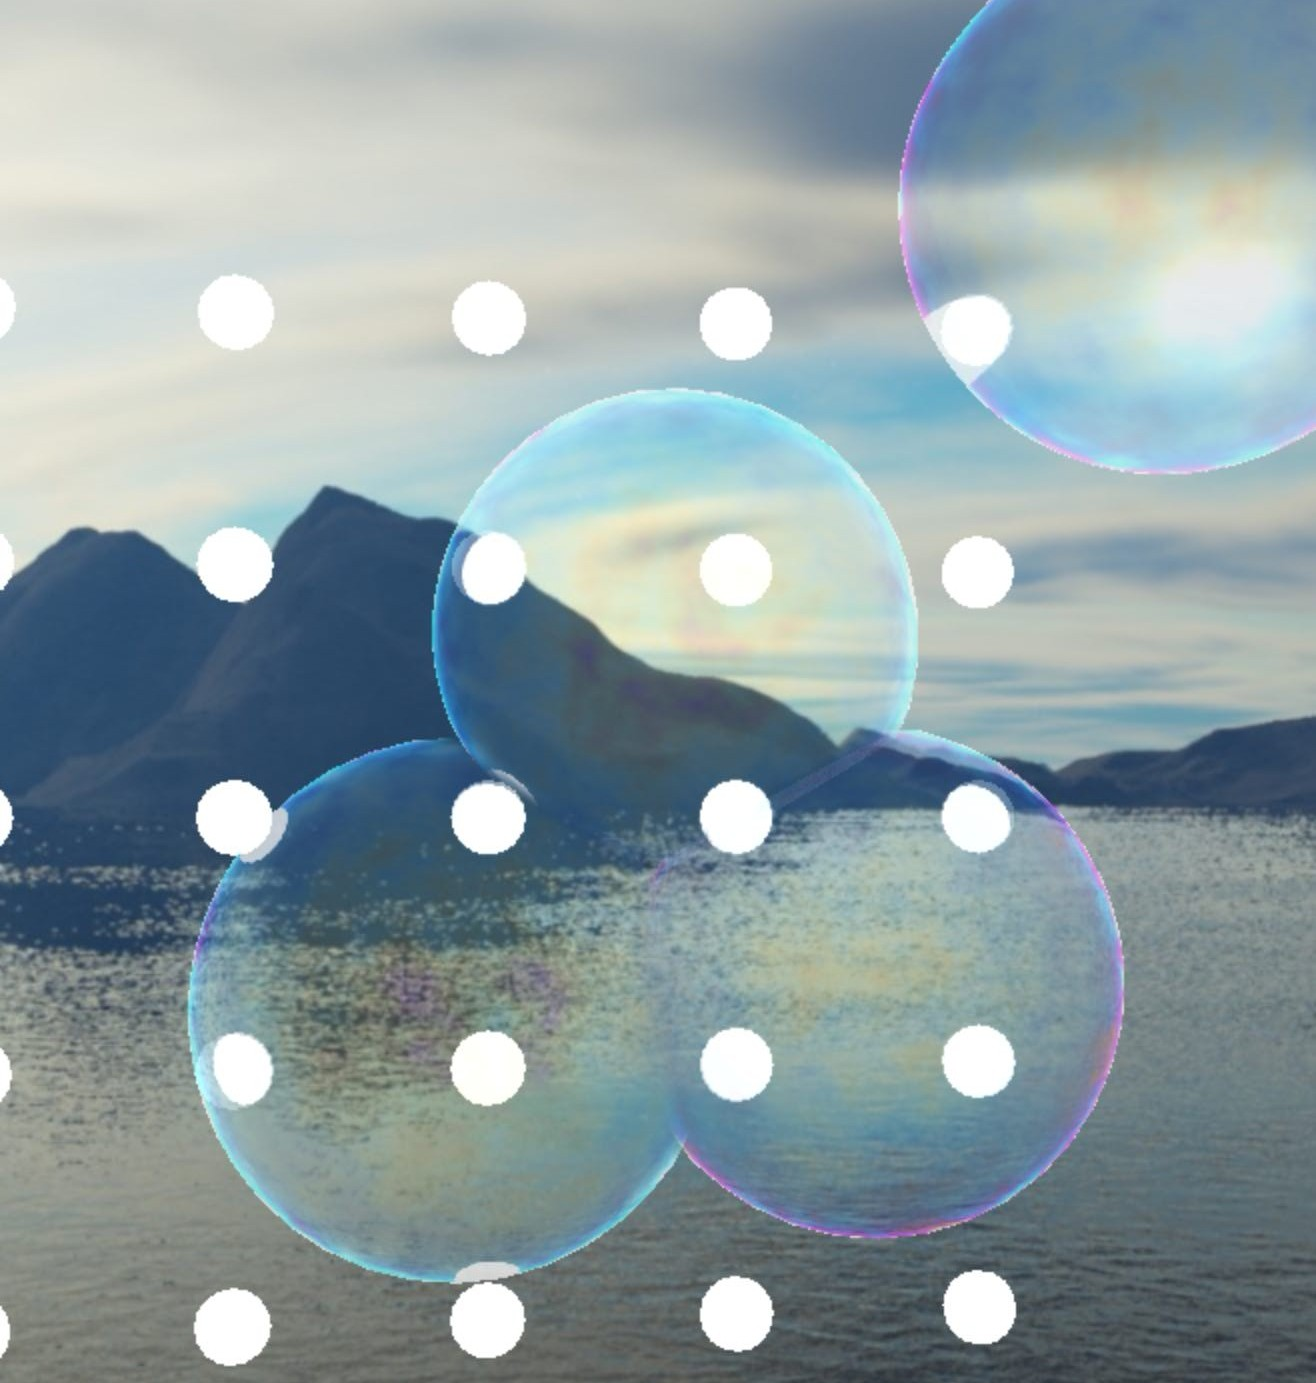
\includegraphics[width=\linewidth]{figures/2.3left.jpg}\\[0.4em]
    \small Kim2012
  \end{minipage}
  \begin{minipage}[t]{0.32\linewidth}
    \centering
    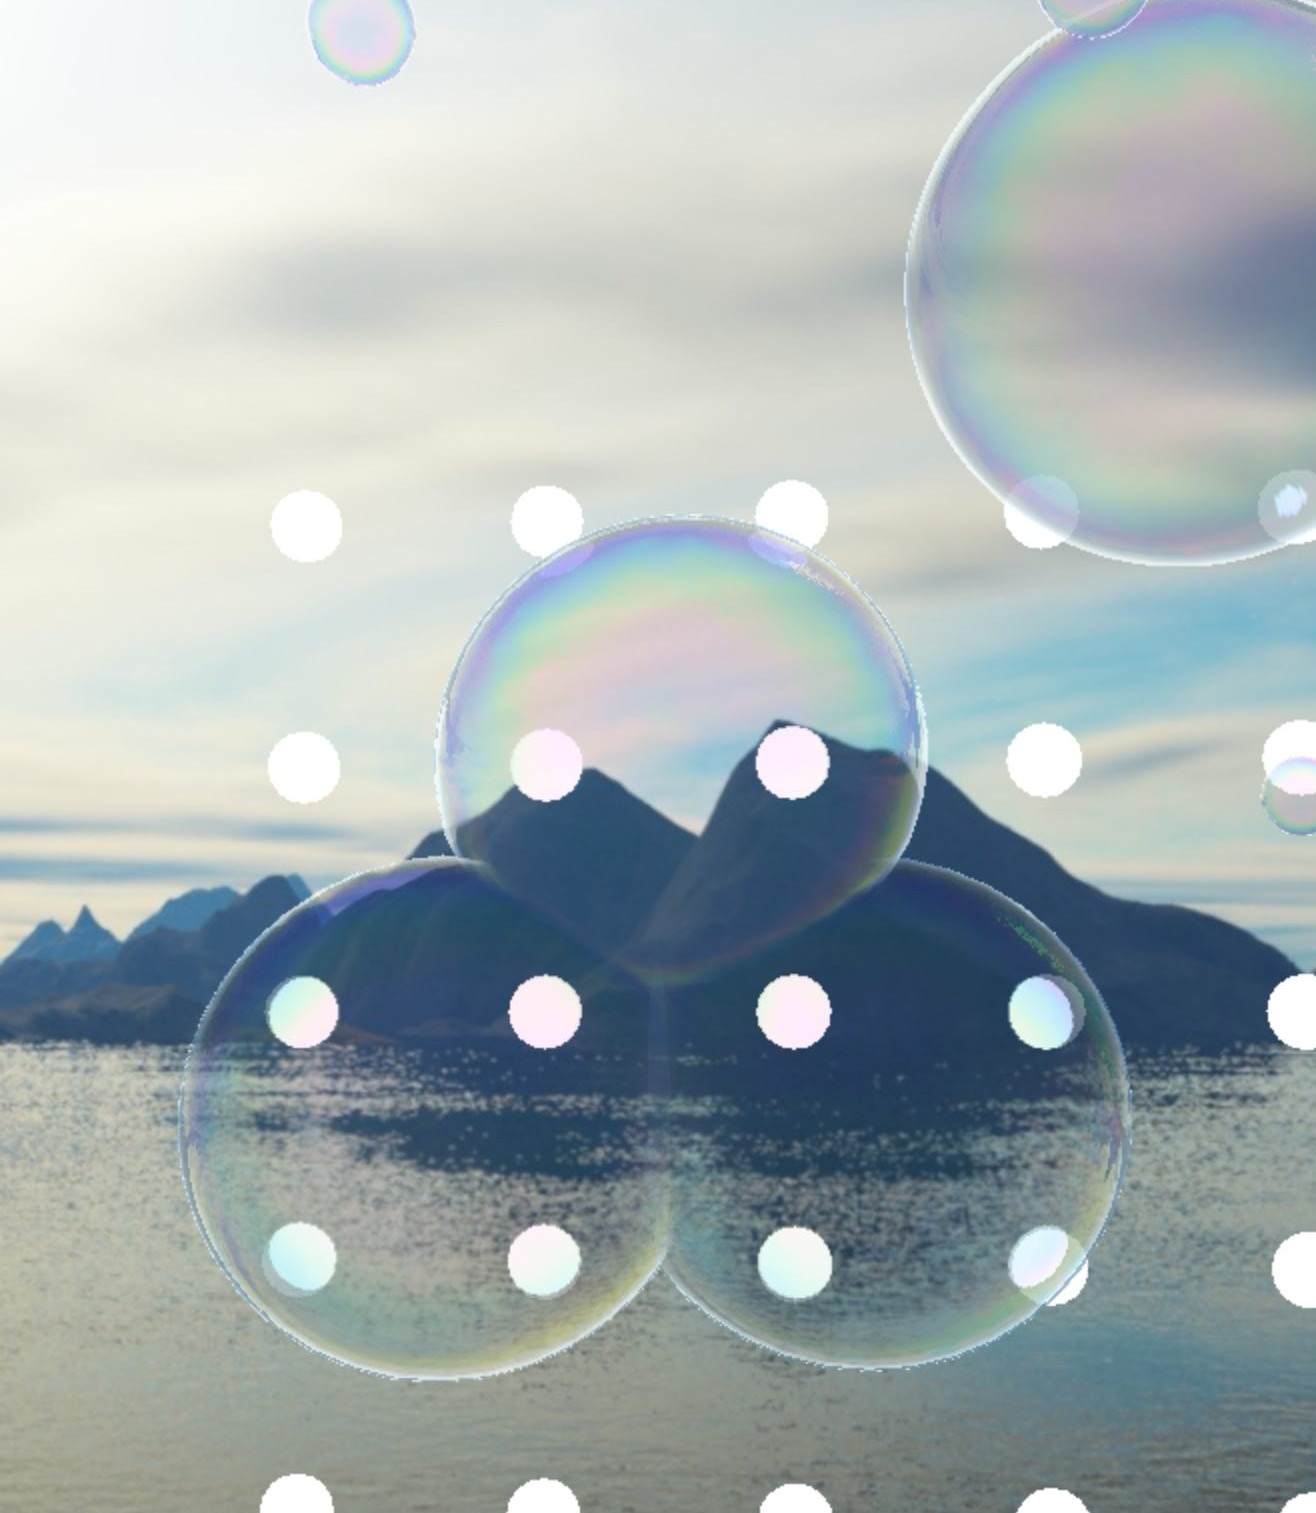
\includegraphics[width=\linewidth]{figures/2.3right.jpg}\\[0.4em]
    \small Belcour Airy
  \end{minipage}
  \caption{不同虹彩模式对比}
  \label{fig:three_modes}
\end{figure}

\section{动态膜厚与颜色合成}

\subsection{动态膜厚}

真实肥皂泡的膜厚会因为重力排液、表面流动和扰动而变化。完整的膜厚动力学可以基于表面上的流体方程建模 \cite{ishida2020thickness}。本项目为了满足移动端实时演示要求，采用 shader 中的程序化近似：使用世界法线方向作为膜面参数，叠加多层 Simplex noise、缓慢流动项、细节噪声和上下方向的排液趋势。

动态厚度可概括为：

\[
d =
d_0
+ A_{\mathrm{var}} P(\mathbf{n}, t)
+ 190 M_{\mathrm{touch}}
+ 95 Q_{\mathrm{ripple}},
\]

其中 $d_0$ 是基础膜厚，$A_{\mathrm{var}}$ 是膜厚变化幅度，$P(\mathbf{n},t)$ 是由多层噪声和排液项组合的厚度图案，其中 $d_0$ 是基础膜厚，$A_{\mathrm{var}}$ 是膜厚变化幅度，$P(\mathbf{n},t)$ 是由多层噪声和排液项组合的厚度图案。

一个重要实现细节是：项目使用 \codepath{normalize(vWorldNormal)} 作为噪声输入方向，而不是使用 UV 坐标。这样可以避免球体 UV 接缝处出现明显断裂，让虹彩流动更连续。

\subsection{颜色合成}

泡泡最终颜色由三部分组成：

\begin{enumerate}
  \item \textbf{透射背景}：从背景 FBO 或背面 FBO 中折射采样得到 \codepath{bgColor}。
  \item \textbf{薄膜虹彩}：由当前模式计算得到 \codepath{filmReflectance}，再根据 Fresnel 边缘项增强。
  \item \textbf{环境反射和高光}：通过 cubemap 采样环境反射，并用薄膜反射率染色；另外加入少量 Blinn-Phong 高光。
\end{enumerate}

中心区域透明度更高，轮廓处透明度下降、反射和虹彩增强。shader 中用

\[
F = (1 - |\mathbf{V}\cdot\mathbf{N}|)^{p}
\]

作为 Fresnel 边缘项，其中 $p$ 对应可调参数 \codepath{uFresnelPower}。这使泡泡中心能保持清透，边缘能呈现更明显的彩色轮廓。


\chapter{物理模拟与动力学}


肥皂泡的本质是浸没在环境空气中的一个极薄液膜，其动力学行为主要由液膜的表面张力、周围空气的不可压缩性，以及空气的惯性主导。传统的基于体积的多相纳维-斯托克斯（Navier-Stokes）求解器虽然能够精确模拟这些现象，但需要大量的计算资源来解析泡泡内部的空气动力学以及薄至微米级的薄膜几何形状。

本项目的方法参考Da 等人提出的 \textit{Double Bubbles Sans Toil and Trouble: Discrete Circulation-Preserving Vortex Sheets for Soap Films and Foams} \cite{da2015doublebubbles}的思路，仅将建模工作集中在泡泡表面。该论文首次提出了一种基于非流形涡流片（vortex sheet）方程来模拟肥皂膜、泡泡和泡沫动力学的数值方法。本项目在其理论基础上实现了一个简化版本，专门用于单个闭合泡泡的动态表面演化。

\section{涡流片模型的理论基础}

涡流片是一个浸没在三维空间中的表面，它界定了速度场切向分量的不连续性——穿过薄片时，速度的切向分量发生跳跃，而法向分量保持连续。这一数学结构恰好契合肥皂膜的物理本质：薄膜两侧分别是内部空气和外部空气，两侧的速度场可以不同，但空气不能穿透薄膜。

DBSTT 方法使用一个标量场——\textbf{环量（circulation）}$\Gamma$——作为描述涡流片状态的主要变量。对于表面上的每一个点 $f(X)$，其环量值定义为沿着一个从固定参考点 $x_0$ 到该点、且穿透薄片的任意闭合环路的环路积分：

\begin{equation}
\Gamma(X) = \oint_L \mathbf{u} \cdot d\mathbf{x}
\label{eq:circulation_def}
\end{equation}

其中 $\mathbf{u}$ 为环境空气的速度场。这一积分的值与环路 $L$ 的具体形状无关（只要它仅在 $x_0$ 和 $f(X)$ 两处穿透薄片），这保证了 $\Gamma$ 是表面上的良定义的标量场。

给定环量场之后，可以分两步恢复速度场。首先计算涡流片强度$\boldsymbol{\gamma}$：

\begin{equation}
\boldsymbol{\gamma} = \mathbf{n} \times \nabla_{\!f}\, \Gamma
\label{eq:vortex_sheet_strength}
\end{equation}

其中 $\mathbf{n}$ 为表面单位法线，$\nabla_{\!f}$ 为表面梯度算子。

接着，通过Biot-Savart积分恢复环境速度场：

\begin{equation}
\mathbf{u}(\mathbf{x}) = \frac{1}{4\pi} \int_S \boldsymbol{\gamma}(\mathbf{x}') \times \frac{\mathbf{x} - \mathbf{x}'}{|\mathbf{x} - \mathbf{x}'|^3} \, df'
\label{eq:biot_savart}
\end{equation}

$\mathbf{u}$ 自动满足 $\nabla \cdot \mathbf{u} = 0$ 。这意味着基于涡流片运动学导出的速度场能够自然地捕捉不可压缩流体的动力学特征，而无需像传统网格方法那样在每步显式求解压力-泊松方程来强制不可压缩性。

下面考虑表面张力驱动的环量演化。在不受外力作用时，根据开尔文环量定理，环量随物质平流守恒：$D\Gamma/Dt = 0$。而由于表面张力的存在，环量场会按照一个简洁的局部定律演化。

考虑不可压缩欧拉方程在涡流片两侧的极限形式，结合表面张力产生的压力跳跃 $p_1 - p_2 = \sigma(H_1 - H_2)$（其中 $\sigma$ 为表面张力系数，$H_1, H_2$ 分别为薄膜两侧的有符号标量平均曲率），可以得到环量演化的核心方程：

\begin{equation}
\frac{D\Gamma}{Dt} = -\frac{\sigma}{\rho} (H_1 - H_2)
\label{eq:circulation_evolution}
\end{equation}

其中 $\rho$ 为空气密度。对于闭合的单个泡泡，两侧的几何重合但朝向相反，因此 $H_1 = -H_2$，从而 $H_1 - H_2 = 2H$。这意味着\textbf{环量的时间变化率与表面的有符号标量平均曲率成正比}——表面曲率大的区域环量变化快，曲率小的区域变化慢。表面张力正是通过这一机制驱动泡泡表面趋向平衡态（对闭合泡泡而言是球面，其上各点曲率相等）。

\section{离散化与数值实现}

将上述连续理论转化为数值算法，需要在空间和时间维度上进行离散化。以下详细介绍本项目在 \codepath{VortexSheetSimulation} 类中的实现。

使用三角网格来表示泡泡表面，在顶点上采样环量场。项目定义了 \codepath{SimMesh} 结构来承载模拟所需的所有数据：

\begin{itemize}
  \item \codepath{positions}：顶点三维位置 $\mathbf{p}_i \in \mathbb{R}^3$
  \item \codepath{triangles}：三角形索引三元组 $(i_0, i_1, i_2)$
  \item \codepath{circulation}：逐顶点存储的标量环量 $\Gamma_i \in \mathbb{R}$
  \item \codepath{vertexNormals}：顶点法线 $\mathbf{n}_i$（通过角度加权平均求出）
  \item \codepath{voronoiAreas}：顶点 Voronoi 对偶面积 $A_i$
  \item \codepath{meanCurvature}：逐顶点有符号标量平均曲率 $H_i$
  \item \codepath{velocity}：逐顶点的诱导速度 $\mathbf{u}_i$
\end{itemize}

初始几何由 \codepath{initIcosphere()} 构建：程序首先生成一个单位二十面体，再通过 midpoint 方式对 icosphere 做指定次数的细分，最后归一化到指定半径 $R = 1.5$。为了触发动力学演化，程序沿一个固定拉伸轴施加初始顶点扰动；在当前鸿蒙提交版本中，应用层设置的扰动幅度为 $16\%$。环量场初始化为全零，法线和面积在初始化完成后立即计算。

\textbf{算法总览}

每次仿真更新遵循 DBSTT 论文\cite{da2015doublebubbles} Algorithm 1 的时间积分循环，经过本项目简化适配后的子步更新流程为：

\begin{enumerate}
  \item \textbf{几何量计算}：\codepath{computeVertexNormalsAndAreas()} + \codepath{computeMeanCurvature()}
  \item \textbf{表面张力积分}：\codepath{integrateSurfaceTension(dt)}
  \item \textbf{环量扩散}：\codepath{diffuseCirculation()}
  \item \textbf{涡流片强度计算}：\codepath{computeVortexSheetStrength(gamma)}
  \item \textbf{毕奥-萨伐尔速度求解}：\codepath{computeBiotSavartVelocities(gamma)}
  \item \textbf{位置推进}：\codepath{advectPositions(dt)}
\end{enumerate}

\codepath{VortexSheetSimulation} 类内部保留了 \codepath{substepsPerFrame = 5}、\codepath{timeStep = 0.0005f} 的默认配置，但当前鸿蒙提交版本在初始化与重置时都会显式改写为 \codepath{substepsPerFrame = 1}、\codepath{timeStep = 0.001f}。同时，Native 渲染层并不是每一帧都推进仿真，而是每隔 \codepath{kSimFrameInterval = 6} 帧调用一次 \codepath{g\_Sim.update(1.0f / 60.0f)}。因此，当前系统中一次实际仿真更新只执行 1 个子步，子步时间步长为 $\Delta t = 0.001$ 秒，子步结束后重新计算法线以供渲染使用。

\textbf{顶点法线与Voronoi面积计算}

顶点法线采用角度加权平均法计算。对每个入射到顶点 $v$ 的三角形面，计算该面的单位法线 $\mathbf{n}_f$，并将其按该三角形在顶点处的内角加权累加：

\begin{equation}
\mathbf{n}_v = \frac{\sum_{f \in \text{faces}(v)} \alpha_f \cdot \mathbf{n}_f}
                 {\bigl\| \sum_{f \in \text{faces}(v)} \alpha_f \cdot \mathbf{n}_f \bigr\|}
\label{eq:angle_weighted_normal}
\end{equation}

其中 $\alpha_f$ 为面 $f$ 中位于顶点 $v$ 处的内角，通过相邻边向量的点积与反余弦求得。对于退化情况（法线长度接近于零），则退化为从原点指向顶点的径向方向。

Voronoi 面积通过将每个入射三角形的面积三等分并累加到其三个顶点上来近似计算。

\textbf{离散平均曲率}

对于标量平均曲率的离散化，本项目参考论文的建议，采用基于边的离散曲率公式：对每对相邻顶点 $(v_i, v_j)$（即每条共享两个三角形的边），计算该边上的积分平均曲率，再均匀分配到其两个端点。具体来说，对于连接 $v_i, v_j$ 的边，假设它由两个三角形 $t_0, t_1$ 共享：

\begin{equation}
\mathbf{K}_i = -\frac{1}{4A_i} \sum_{j \in \mathcal{N}(i)} (\cot\alpha_{ij} + \cot\beta_{ij})\,(\mathbf{p}_j - \mathbf{p}_i)
\label{eq:cotan_curvature}
\end{equation}

其中 $A_i$ 为顶点 $v_i$ 的 Voronoi 面积，$\mathcal{N}(i)$ 为 $v_i$ 的一环邻域，$\alpha_{ij}, \beta_{ij}$ 分别为边 $e_{ij}$ 在两个入射三角形中对面的两个角。$\cot\alpha$ 通过边向量的点积除以叉积模长求得：

\begin{equation}
\cot\alpha = \frac{\mathbf{e}_{ik} \cdot \mathbf{e}_{jk}}{\|\mathbf{e}_{ik} \times \mathbf{e}_{jk}\|}
\label{eq:cotan}
\end{equation}

在代码实现中，程序首先构建从边到其入射面列表的映射，然后仅处理恰好由两个三角形共享的边，计算两侧的余切权重并累加到曲率法线 $\mathbf{K}_i$ 上。最终的标量平均曲率通过对曲率法线取负点积获得：

\begin{equation}
H_i = -\mathbf{K}_i \cdot \mathbf{n}_i
\label{eq:scalar_H}
\end{equation}

负号确保了向外法线约定下的符号正确性：在凸区域（如球面），$\mathbf{K}$ 指向内侧，与向外法线 $\mathbf{n}$ 的点积为负，取负后 $H > 0$。

\textbf{表面张力积分}

有了每个顶点的离散标量平均曲率 $H_i$，就可以根据方程 (\ref{eq:circulation_evolution}) 对环量进行前向欧拉更新。对于单个闭合泡泡，两侧界面几何重合但朝向相反：$H_1 = H, H_2 = -H$，故 $H_1 - H_2 = 2H$。离散更新公式为：

\begin{equation}
\Delta\Gamma_i = \text{sign} \cdot \frac{\sigma}{\rho} \cdot \Delta t \cdot 2 \cdot H_i
\label{eq:discrete_dGamma}
\end{equation}

其中 $\sigma/\rho$ 对应代码中的 \codepath{surfaceTensionStrength}（默认值 $15.0$），$\text{sign}$ 通过 \codepath{flipSurfaceTensionSign}（默认 \codepath{true}，即取正号）控制。

值得注意的是，论文中原本的公式包含顶点面积 $A_v$ 在分母中，但由于我们使用逐点的 $H_i$ 而非积分的曲率 $H_i^v$，$A_v$ 在分子分母中恰好抵消简化。

\textbf{Vortex Sheet Strength 计算}

环量更新完成后，需要在每个三角形上计算涡流片强度 $\boldsymbol{\gamma}$。根据方程 (\ref{eq:vortex_sheet_strength})，$\boldsymbol{\gamma} = \mathbf{n} \times \nabla_{\!f}\,\Gamma$。在三角形 $t = (v_0, v_1, v_2)$ 上，环量场是分段线性的，其表面梯度为常数。代码实现使用三角形三个顶点的环量值来计算梯度：

\begin{equation}
\boldsymbol{\gamma}_t = \mathbf{n}_t \times \frac{
    \Gamma_0 (\mathbf{p}_2 - \mathbf{p}_1) +
    \Gamma_1 (\mathbf{p}_0 - \mathbf{p}_2) +
    \Gamma_2 (\mathbf{p}_1 - \mathbf{p}_0)
}{2 \cdot \text{area}(t)}
\label{eq:discrete_gamma}
\end{equation}

其中 $\mathbf{n}_t$ 为三角形面的单位法线，通过边向量的叉积归一化得到，且保证与从原点指向三角形质心的方向一致（向外朝向）。

\textbf{正则化毕奥-萨伐尔速度求解}

对于每个顶点 $v_i$，需要计算所有三角形 $t_j$ 对其诱导速度的贡献之和。为避免距离趋近于零时的奇异性，DBSTT 采用 正则化形式：

\begin{equation}
\mathbf{u}(\mathbf{x}) = \frac{1}{4\pi} \sum_{t} \boldsymbol{\gamma}_t \times
    \frac{\mathbf{x} - \mathbf{c}_t}
         {(|\mathbf{x} - \mathbf{c}_t|^2 + \alpha^2)^{3/2}} \cdot A_t
\label{eq:regularized_biot_savart}
\end{equation}

其中 $\mathbf{c}_t$ 为三角形 $t$ 的质心，$A_t$ 为其面积，$\alpha$ 为正则化参数。代码中 $\alpha$ 自动设为网格平均边长（在初始化时计算）的 $1.0$ 倍，即 \codepath{regularizationAlpha = avgEdgeLength * 1.0f}。

实现细节上，程序预计算每个三角形的质心、面积和 $\boldsymbol{\gamma}_t$ 值，然后对每个顶点遍历所有三角形，进行双重循环求和。每个贡献项为 $\boldsymbol{\gamma}_t \times \mathbf{r}$ 乘以面积和分母幂次的倒数，其中 $\mathbf{r} = \mathbf{x} - \mathbf{c}_t$ 为从三角形质心到当前顶点的向量。最终速度除以 $4\pi$ 以匹配连续积分中的系数。

\textbf{位置推进与安全钳制}

顶点位置使用前向欧拉法更新：$\mathbf{p}_i \leftarrow \mathbf{p}_i + \mathbf{u}_i \cdot \Delta t$。为确保稳定性，代码施加了一个位移上限，限制每个子步的顶点位移不超过平均边长的 $10\%$：

\begin{equation}
\|\Delta\mathbf{p}_i\|_{\max} = 0.1 \cdot \bar{e}
\label{eq:max_displacement}
\end{equation}

其中 $\bar{e}$ 为平均边长。这是为了解决调试代码过程中出现的因数值不稳定导致的网格穿刺或顶点飞散问题。

位置更新后，所有顶点统一减去网格质心，以防止因数值漂移导致的整体平移，保持毕奥-萨伐尔积分的对称性。

\textbf{环量扩散}

为了进一步抑制数值不稳定性，代码在每个子步中施加一个轻微的拉普拉斯扩散：

\begin{equation}
\Gamma_i \leftarrow \Gamma_i + \nu \cdot \frac{1}{|\mathcal{N}(i)|} \sum_{j \in \mathcal{N}(i)} (\Gamma_j - \Gamma_i)
\label{eq:circulation_diffusion}
\end{equation}

其中 $\nu$ 为扩散系数，默认值 \codepath{circulationDiffusion = 0.0005}，非常小，仅用于消除高频数值振荡而不影响宏观动力学行为。DBSTT 论文也指出，这种扩散可以解释为对空气粘度的合理视觉近似。

\section{与本项目渲染管线的集成}

物理模拟与渲染管线的衔接位于 \codepath{RenderFrame()} 函数中：

\begin{enumerate}
  \item 渲染循环开始后，若模拟未被暂停（\codepath{g\_SimPaused == false}），则每隔 \codepath{kSimFrameInterval = 6} 帧调用一次 \codepath{g\_Sim.update(1.0f/60.0f)}，按较低频率推进一次仿真更新。
  \item 模拟完成后，调用 \codepath{buildVerticesFromSim()} 将 \codepath{SimMesh} 中的顶点位置和法线转换为 GPU 可用的 \codepath{Vertex} 数组。
  \item 通过 \codepath{Mesh::updateVertices()} 将更新后的顶点数据上传至 OpenGL VBO，后续的折射/虹彩 shader 即可使用变形后的几何体进行渲染。
\end{enumerate}

主泡泡的模型矩阵保持为单位矩阵，所有变形信息完全包含在经模拟更新的顶点位置中，这使得 shader 中的法线计算能够正确地反映泡泡表面的动态形变。

当前实现没有加入原论文中的完整非流形拓扑变化、泡沫多区域标记和线框约束，只是一个 DBSTT 风格的单泡泡表面动态近似。它的作用是让主泡泡轮廓和表面法线随时间发生微小变化，从而让折射和虹彩不显得完全静止。      

具体动态效果详见项目演示视频。可以明显观察到主泡泡在当前系统中保持持续的小幅表面形变，并在参数调整后呈现不同强度的恢复趋势。


\chapter{交互与演示}
\section{交互实现}

\subsection{触控交互}

当前系统以 HarmonyOS 触控为主要交互方式，最核心的演示路径由三类手势构成：

\begin{table}[H]
  \centering
  \caption{触控交互}
  \begin{tabular}{p{0.24\linewidth}p{0.64\linewidth}}
    \toprule
    操作 & 效果 \\
    \midrule
    单指拖动 & 改变相机 yaw/pitch，围绕泡泡观察。\\
    双指缩放 & 改变相机距离，实现缩放。\\
    单指点击/短按 & 在主泡泡上产生局部膜厚增强和环形折射波纹。\\
    \bottomrule
  \end{tabular}
\end{table}

在页面层，ArkTS 会先根据 XComponent 的实际区域将输入事件映射到局部坐标，再通过 NAPI 把坐标、事件类型和视口尺寸传给 Native 渲染层。单指点击主泡泡时，程序把触摸位置转换为归一化屏幕坐标 \codepath{g\_TouchPoint}，并记录触摸强度与局部移动速度 \codepath{g\_TouchVelocity}。当单指移动超过较小阈值后，ArkTS 侧会优先把后续移动解释为 \codepath{rotateCamera()} 输入，因此连续大幅拖动并不是局部波纹的主要触发方式。shader 中计算当前 fragment 到触摸点的距离：

\[
r = \left\|\mathbf{u}_{\mathrm{frag}}-\mathbf{u}_{\mathrm{touch}}\right\|.
\]

局部触摸强度采用高斯型衰减：

\[
M_{\mathrm{touch}} =
\exp\left(-\frac{r^2}{0.0065}\right) S_{\mathrm{touch}},
\]

环形波纹采用正弦函数叠加指数衰减：

\[
Q_{\mathrm{ripple}} =
\sin(78r - 18t)\,\exp(-9r)\,S_{\mathrm{touch}}
(0.35+0.65V_{\mathrm{touch}}).
\]

触摸只作用在主泡泡上。绘制展示泡泡时，程序向 shader 传入无效触摸点和零强度，避免副泡泡受到局部触摸扰动。由于这一部分的效果高度依赖连续交互，具体动态表现以比赛提交视频中的演示为准。

\subsection{界面参数}

系统将主要控制项整理为移动端界面按钮和参数面板，使评审能够直接在鸿蒙设备上观察到参数变化。当前界面主要包含模式切换、仿真控制和参数滑条三类入口：

\begin{table}[H]
  \centering
  \caption{界面参数控制}
  \begin{tabular}{p{0.20\linewidth}p{0.26\linewidth}p{0.42\linewidth}}
    \toprule
    界面项 & 参数 & 作用 \\
    \midrule
    模式按钮 & Kim / Airy & 切换两种主要演示模式；Native 层仍保留 Spectral LUT 便于内部对比。\\
    状态按钮 & 暂停仿真 / 重置 & 暂停或继续主泡泡表面模拟，并同步冻结或恢复基于时间的视觉变化；重置时恢复默认参数。\\
    光学参数 & 干涉膜厚、折射强度、环境反射 & 调整彩色条纹尺度、背景扭曲强度和环境反射权重。\\
    仿真参数 & 厚度扰动、表面张力、边缘畸变 & 调整动态膜厚幅度、主泡泡恢复趋势和轮廓额外折射增强。\\
    视图参数 & 相机距离 & 调整观察远近，便于展示单泡泡细节或多泡泡整体构图。\\
    状态显示 & FPS、当前模式、交互提示 & 方便现场展示系统帧率、当前材质模式和操作说明。\\
    \bottomrule
  \end{tabular}
\end{table}

除 ArkTS 界面当前开放的滑条外，Native 接口层还保留了 \codepath{uFresnelPower} 与 \codepath{uMaxOffsetRatio} 对应的调节入口，用于内部调参与折射稳定性验证；它们没有直接暴露在比赛演示面板中。

这些参数直接服务于最终鸿蒙版本的展示与调参流程。具体调节过程和实时反馈可参考演示视频。

\chapter{结果与分析}
\section{结果分析与局限}

当前系统已经实现了面向比赛提交和现场演示的 HarmonyOS 透明泡泡渲染效果。主要结果包括：

\begin{itemize}
  \item 通过多阶段 FBO 近似双界面折射，背景参照物和天空盒能在泡泡中产生明显扭曲。
  \item 两种薄膜虹彩模式已经在 Native 层实现，界面开放 Kim 与 Airy 两种展示模式，便于说明实时公式与多波长近似之间的差异。
  \item 动态膜厚让虹彩随时间缓慢流动，不依赖静态纹理。
  \item 触摸交互能够产生局部膜厚增强和波纹，配合参数面板形成更自然的现场展示反馈。
  \item 主泡泡接入 DBSTT/vortex sheet 风格表面动态，16 个多展示泡泡通过距离排序与 Alpha 混合合成，用于丰富空间构图与比赛演示层次。
  \item ArkTS 页面、NAPI 接口、Native 渲染层和可执行 HAP 程序已经形成完整的提交链路。
\end{itemize}

同时，系统也有明确局限：

\begin{itemize}
  \item 屏幕空间折射不能表现屏幕外物体，也不能严格模拟多泡泡之间的相互折射。
  \item Belcour Airy 模式是实时 shader 中的项目级简化，不包含完整微表面模型和解析光谱预积分。
  \item 动态膜厚主要由噪声、排液趋势和触摸扰动驱动，没有求解完整的薄膜厚度流体方程。
  \item DBSTT 模拟只用于单个闭合泡泡，不支持原论文中的泡沫拓扑变化和 Plateau 边界。
  \item 展示泡泡只做视觉漂移，不参与主泡泡的物理碰撞或流体耦合。
\end{itemize}

如果继续迭代比赛版本，后续优先考虑补强多泡泡之间的相互折射、碰撞与排序一致性，并进一步完善移动端性能记录。

\section{总结}

本项目从透明肥皂泡的主要视觉现象出发，实现了一个面向赛题二提交的 HarmonyOS 渲染系统。渲染方面，项目通过多阶段 FBO 合成近似双界面折射，并用低分辨率 FBO 与坐标修正兼顾移动端性能和多泡泡显示稳定性。光学方面，项目实现了 Kim2012和Belcour Airy 两种薄膜虹彩模式，能够展示实时公式计算、预计算纹理和多波长 Airy 近似之间的差异。动态方面，项目结合程序化膜厚变化、触摸波纹、DBSTT 风格主泡泡形变和多泡泡风吹漂移，使最终结果更符合比赛对“效果、交互、完整性”的要求。

后续如继续扩展该项目，可进一步加入更严格的光谱到 RGB 积分、更真实的膜厚流体模拟、多泡泡之间的相互折射和碰撞，以及基于体积或拓扑变化的泡沫模拟。



\bibliography{bib/soapbubble}  % 参考文献使用 BibTeX 编译
% \printbibliography       % 参考文献使用 BibLaTeX 编译



\end{document}
